\documentclass{article}
\usepackage[utf8]{inputenc}
\usepackage[a4paper, portrait, margin=0.6in]{geometry}
\usepackage{graphicx}
\usepackage{subcaption}
\usepackage{amsmath}
\usepackage{geometry}
\usepackage{array}


\title{Software Testing (UE18CS400SB) \\ Unit 2}
\author{Aronya Baksy}
\date{September 2021}

\begin{document}
\maketitle

\section{Unit Testing}
\begin{itemize}
    \item Testing of individual units/components of a software to validate that each unit performs as expected
    
    \item Done during implementation phase by developers, and involves white-box testing.
    
    \item Unit: Single function/method/procedure/module/class
    
    \item Reasons for unit testing:
    \begin{enumerate}
        \item Reduces defect costs, saves time and money
        
        \item Increases confidence in code maintenance
        
        \item Enhances reusability, reliability, speed of development
        
        \item Makes debugging easier
    \end{enumerate}
    
    \item Unit testing is of 2 types, \textbf{manual} or \textbf{automated}. 
\end{itemize}
\subsection{How does it work?}
\begin{itemize}
    \item Developer may write test code within the application to test that unit (this test code is commented out during final deployment)
    
    \item Developer may also copy the unit under test to a separate environment and test it in isolation. This is more rigorous and reveals unnecessary dependencies between units.
    
    \item Developer uses unit test framework to develop automated test cases. Each test consists of critera to verify the correctness of the code. Failed test cases are logged and reported
\end{itemize}

\subsection{Unit Test Techniques}
\begin{itemize}
    \item \textbf{Black-Box}: Test of user interface, input and output
    
    \item \textbf{White-Box}: Testing functional behaviour of the application
    
    \item \textbf{Grey-Box}: Used to execute test suites/methods/cases and perform risk analysis
\end{itemize}

\subsection{Advantages}
\begin{itemize}
    \item Unit tests allow new team members to quickly understand the unit and the project API
    
    \item Ensures that units function normally even after refactoring (a.k.a regression testing)
    
    \item Units can be tested in parallel independent of the schedule of other units
\end{itemize}

\subsection{Disadvantages}
\begin{itemize}
    \item 100\% branch and condition coverage is not possible, hence all errors may not be caught
    
    \item Errors caused by integration of units cannot be caught by unit tests.
\end{itemize}

\subsection{Test-Driven Development}
\begin{itemize}
    \item Rules of TDD:
    \begin{enumerate}
        \item Before writing code, write a failing test case
        
        \item Remove all duplicates
    \end{enumerate}
\end{itemize}
\begin{figure}[!ht]
    \centering
    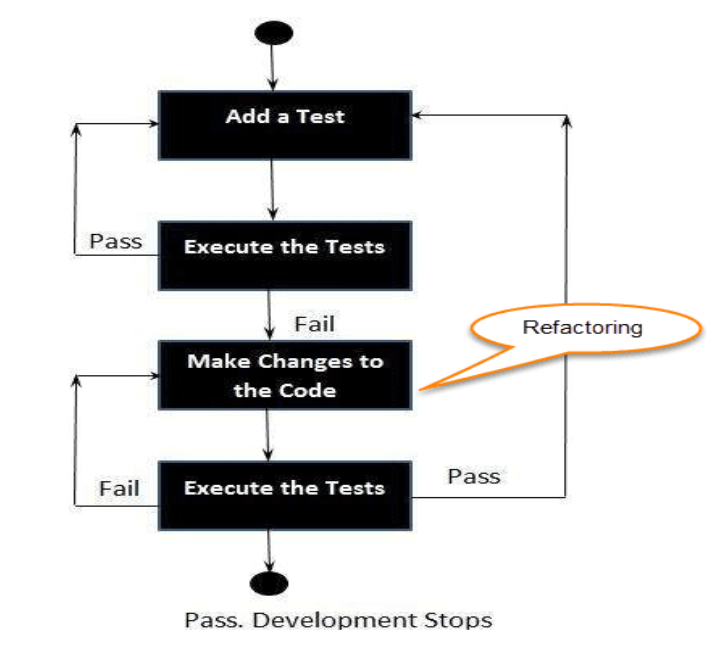
\includegraphics[scale=0.5]{st1.png}
    \caption{Test-Driven Development}
    \label{fig:my_label}
\end{figure}

\begin{itemize}
    \item Advantages of TDD:
    \begin{enumerate}
        \item It promotes affirmative testing of the application and its specifications.
        
        \item Makes code simpler and clear.

        \item Reduces the documentation process at developers end.
    \end{enumerate}
\end{itemize}

\subsection{Unit Testing Checklist}
\begin{itemize}
    \item Write unit tests for every unit
    
    \item Don't postpone unit tests, perform them immediately
    
    \item Ensure that code passes unit and integration tests before checking it in to the source control
    
    \item Use automated tools like JUnit and NUnit for unit testing
    
    \item Check test files and assets related to testing into the source control
    
    \item Use test driven development for maximum coverage
    
    \item Refactor the code only when thorough tests are available
\end{itemize}

\section{White-Box Testing}
\begin{itemize}
    \item Testing based on knowledge of the software's internal workings
    
    \item Focus: strengthening quality of implementation proving design and usability
    
    \item Requires mapping between program code and actual functionality
    
    \item Why: early defect identification, confidence building, reduces complexity of further testing, addresses both functional and non-functional aspects
\end{itemize}
\subsection{Objectives of White Box Testing}
\begin{itemize}
    \item Finding Broken or poorly structured paths in the coding processes
    \item The flow of specific inputs through the code
    \item Defects due to common programming mistakes and common security holes
    \item Testing of each statement, object and function on an individual basis
\end{itemize}

\section{Static Testing}
\begin{itemize}
    \item Analysis of code either by human or by tool (no executables involved)
    
    \item Aspects: 
    \begin{enumerate}
        \item Works according to requirements, does not miss any functionality
        
        \item Code is according to architecture developed eariler
        
        \item Error and exception handling
        
        \item Follows coding standards, professional best practices 
    \end{enumerate}
    
    \item Humans can compare code more accurately with the specification, identify root causes, and special/rare conditions
\end{itemize}

\subsection{Types of Static Testing}
\subsubsection{Desk Checking}
\begin{itemize}
    \item Informal check against specifications (no formalisms, no structure, no documentation maintained)
    
    \item Performed by the code author
    
    \item Suffices for programming errors, but may not work for incomplete/misunderstood requirements
    
    \item \textbf{Advantages}: Programmers know the code in and out hence suited to do testing, less logistics needed, reduced delays in defect detection and correction
    
    \item \textbf{Disadvantages}: Developers are narrow minded, don't like testing, and process is not scalable/reproducible
\end{itemize}

\subsubsection{Code Walkthrough}
\begin{itemize}
    \item Group oriented, brings in multiple perspectives, each having their own role (Fagan Inspection)
    
    \item Highly formal, structured, participants have clear roles, diverse views
    
    \item \textbf{Roles}:
    \begin{itemize}
        \item \textbf{Author}: writes code, fixes defects
        
        \item \textbf{Moderator}: controls meetings
        
        \item \textbf{Reviewers}: Read documentation before meeting, report defects
        
        \item \textbf{Scribe}: Take notes during meetings, documents the minutes of the meeting
    \end{itemize}
    
    \item Fagan inspection process: Planning, overview, individual prep, meeting, re-work, follow-up
    
    \item \textbf{Advantages}: Thorough inspection, multiple perspectives, real-world effective
    
    \item \textbf{Disadvantages}: Lots of logistics, time consuming, full code coverage is hard
\end{itemize}

\subsection{Tool-driven Static Testing}
\begin{itemize}
    \item Static analysis tools uncover the following:
    \begin{enumerate}
        \item Unreachable code
        
        \item Unused but declared variables, not-freed dynamically allocated memory
        
        \item Type errors related to unsafe type casting
        
        \item Non-portable code, code that does not adhere to standards
        
        \item Errors related to coding guidelines: naming conventions, indentation, documentation
    \end{enumerate}
    
    \item Cyclomatic complexity is a testing metric that determines the number of independent paths executed
    
    \item Cyclomatic complexity helps to improve code coverage, evaluate risks and ensures that all paths are covered
    
    \item Formula for cyclomatic complexity given a control flow graph $G$ with $E$ edges, $N$ nodes, out of which $P$ nodes are predicate nodes:
    \begin{equation*}
        V(G) = E - N + 2 = P  + 1
    \end{equation*}
\end{itemize}

\section{Structural Testing}
\begin{itemize}
    \item Entails running the executable against a set of test cases, then compare the results with the expected
\end{itemize}
\subsection{Types of Structural Testing}
\subsubsection{Unit Functional Testing}
\begin{itemize}
    \item Initial quick checks by developer, removes "obvious" errors
    
    \item Done at programmer level, uses stubs and harnesses to replace those modules that are not yet implemented
    
    \item Unit testing tools like JUnit are used
\end{itemize}
\subsubsection{Coverage Testing}
\begin{itemize}
    \item Map code to required functionality and cover as much code as possible with test cases
    
    \item Find out percentage of code covered by "instrumentation", identify the most executed critical routines in the code
    
    \item Instrumentation: profiling and logging activites that help in measuring software performance and bugs.
    
    \item Coverage = percentage of statements executed out of the total statements in the program.
    
    \item Types: statement, path, condition, function coverage
    
    \item Test for sequential instructions: generate test cases that cover the entire block of statements, test for asynchronous exceptions and multiple entry points (if present)
    
    \item Test for conditional branch: atleast 1 test case per possible execution path
    
    \item Test for loop statements: Test boundary conditions (0 loop exec, 1 loop exec, Max loop exec, Max-1 loop exec)
    
    \item Path Coverage: provides better representation than sequential coverage (e.g.: in an "if-then-else" statement having 2 test cases, 1 for the True and 1 for False part, each case has only 50\% code coverage)
    
    \item Condition coverage: Refinement of path coverage, makes sure all constituent boolean expressions are covered by testing, protects against compiler optimizations
    
    \item Function coverage: more logical, easy to trace against the RTM, easy to prioritize, easier to achieve full coverage
\end{itemize}

\subsubsection{Complexity Testing}
\begin{itemize}
    \item Number of independent paths in the control flow of the program gives some upper bound on number of tests needed for full coverage
    
    \item Such information is derived from cyclomatic complexity testing
\end{itemize}

\section{Integration Testing}
\begin{itemize}
    \item Testing of components/units after being integrated at any level. Once integrated, the appropriate testing technique is used
    
    \item Integration testing uncovers interfacing problems between components, and functional problems
    
    \item Errors caught in integration test:
    \begin{enumerate}
        \item Interface mismatch: parameters/args, return type, return value, other semantics mismatch
        
        \item Missing interfaces
        
        \item Protocol mismatch across interfaces
        
        \item Error handling across interfaces
    \end{enumerate}
    
    \item Integration errors may or may not manifest themselves in the form of error messages and runtime errors
    
    \item \textbf{Internal interface}: Communication across modules, used only by devs, not exposed to customer
    
    \item \textbf{External interface}: Used by third-party developers to be used by other systems/solutions, need to understand usage and purpose of providing
    
    \item Steps in integration test:
    \begin{enumerate}
        \item Create test cases, test data and test plan
        
        \item test environment setup acc. to test plan
        
        \item Execute test cases and report results
        
        \item Repeat above 2 steps till required (till test adequacy criteria is reached)
        
        \item Repeat till all components have been integrated, use integration tools/scripts where appropriate
    \end{enumerate}
    
\end{itemize}
\subsection{Top-Down Integration}
\begin{itemize}
    \item Approach: integrate high-level components first then low level.
    
    \item If some unit/component not available, "stub" required. 
    
    \item Advantages: Test high level logic and data flow early, early demo of prototypes, coverage improves without changes to test code
    
    \item Disadvantages: Need for stubs, hard to observe data flow, low-level functions are developed later as they don't need testing up front which is bad practice, poor support for early release
\end{itemize}

\subsection{Bottom-Up Integration}
\begin{itemize}
    \item Integrate lower level modules first, then integrate higher and higher level modules
    
    \item Stubs are required to replace unavailable modules
    
    \item Advantages: low-level utilities are tested earlier, less need for stubs, easy to observe data flow
    
    \item Disadvantages: Need for drivers, high-level logic and data flow are tested late, demo is created late, Many loose integration segments to be managed, poor support for early release
\end{itemize}

\subsection{Bi-Directional Integration}
\begin{itemize}
    \item A combination of top-down and bottom up testing, using both stubs (downstream connection) and drivers (upstream connection)
    
    \item Top layers testing uses top-down testing (stubs). Bottom layers are tested using bottom-up testing (drivers)
\end{itemize}

\subsection{Big-Bang System Integration}
\begin{itemize}
    \item Approach in which all software components (modules) are combined at once and make a complicated system. 
    
    \item This combination of different modules is then tested as a single entity. 
    
    \item Ideal when the interfaces are stable and have fewer defects.
\end{itemize}

\subsection{Scenario Testing}
\begin{itemize}
    \item Uses scenarios i.e. speculative stories to help the tester work through a complicated problem or test system. 
    
    \item Scenario characteristics: Story, Motivating, Credible, Complex, Easy to evaluate

    
    \item Possible Strategies to create good scenarios: 
    \begin{enumerate}
        \item Evaluate user actions and objectives, list system events
        
        \item Hacker mindset: try to break the system
        
        \item Study complaints with past systems/competitor systems
    \end{enumerate}
    
    \item Risks of scenario testing:
    \begin{enumerate}
        \item Complex involving many features.
        
        \item Not designed for coverage of the program or for test coverage.
        
        \item Complicated for unstable products
    \end{enumerate}
\end{itemize}
\subsection{Choice of integration method}
\begin{itemize}
    \item Clear requirement and design: top down
    
    \item Dynamic requirement/design/architecture: bottom up
    
    \item Stable design, changing architecture: bi-directional
    
    \item Limited, low-impact changes to architecture: system
    
    \item Combination of above: select one with analysis
\end{itemize}S
\section{System Testing}
\begin{itemize}
    \item Tests a completely integrated system to verify that its compliant with its specified requirements, in the context of a FRS and a SRS
    
    \item Why system test? Provides independent and third-party perspective, holistic and realistic tests, functional and non-funcitonal tests, build confidence and analyze risks, ensure specs are complied with
    
    \item Types of non-functional system testing:
    \begin{enumerate}
        \item Performance testing: execution time in comparision with competitors/different versions
        
        \item Scalability Testing
        
        \item Reliability Testing
        
        \item Stress Testing
        
        \item Interoperability testing
        
        \item L10n and I18n 
    \end{enumerate}
\end{itemize}

\subsection{Functional Testing}
\begin{itemize}
    \item Uses black-box tests to validate the software system against the functional requirements spec (maybe manual or automated)
    
    \item Checks User Interface, APIs, Database, Security, Client/Server communication and other functionality of the Application Under Test
\end{itemize}

\subsection{Non-Functional Testing}
\begin{itemize}
    \item Check non-functional aspects (performance, usability, reliability, etc) of a software application. This affects the client interaction
    
    \item Test the readiness of a system as per nonfunctional parameters which are never addressed by functional testing.
\end{itemize}
\end{document}